\dev{Emile Martinez}{}

\paragraph{Insertion d'un élément dans un tas min} \enspace \newline

\begin{tikzpicture}[-]
	\node[state] (q0) {} ;
	\node[state,below left = 1.1cm and 2.5cm of q0] (q1) {} ;
	\node[state,below right = 1.1cm and 2.5cm of q0] (q2) {} ;
	\node[state,below left = 1.1cm and 1cm of q1] (q3) {} ;
	\node[state,below right = 1.1cm and 1cm of q1] (q4) {} ;
	\node[state,below left = 1.1cm and 1cm of q2] (q5) {} ;
	\node[state,below right = 1.1cm and 1cm of q2] (q6) {} ;
	\node[state,below left = 1.1cm and 0.1cm of q3] (q7) {};
	\node[state,below right = 1.1cm and 0.1cm of q3] (q8) {};
	\node[state,below left = 1.1cm and 0.1cm of q4] (q9) {};
	\node[state,below right = 1.1cm and 0.1cm of q4] (q10) {};
	\node[state,below left = 1.1cm and 0.1cm of q5] (q11) {};
	\node[state,red, below right = 1.1cm and 0.1cm of q5] (q12) {x};
	
	\draw (q0) edge[] node{} (q1);
	\draw (q0) edge[]node{} (q2);
	\draw (q1) edge[]node{} (q3);
	\draw (q1) edge[] node{} (q4);
	\draw (q2) edge[] node{} (q5);
	\draw (q2) edge[] node{} (q6);
	\draw (q3) edge[] node{} (q7);
	\draw (q3) edge[] node{} (q8);
	\draw (q4) edge[] node{} (q9);
	\draw (q4) edge[] node{} (q10);
	\draw (q5) edge[] node{} (q11);
	\draw (q5) edge[red] node{} (q12);
	\draw (q5) edge[<->, bend left, green] node{} (q12);
	\draw (q5) edge[<->, bend left, green] node{} (q2);
\end{tikzpicture}

\paragraph{Notation} Pour $s$ un sommet, un note $p(s)$ le père de $s$ et $\mathcal A_s$ l'arbre enraciné en s. Notons $\mathcal A$ l'arbre global.

\begin{algorithm}[H]
	Mettre x au seul endroit qui préserve la structure de tas\\
	\Tq{$x < p(x)$}
		{Echanger $x$ et $p(x)$}
	\caption{Insertion de dans un tas min}
\end{algorithm}

\paragraph{Correction}
\begin{itemize}
	\item La structure d'arbre presque complet est préservée par l'insertion et par les inversions
	\item Intéressons nous maintenant à la structure de tas.\\
	\\
	On a alors l'invariant de boucle suivant : \begin{itemize}[label = $\circ$]
		\item[« $\circ$] $\mathcal A \setminus \mathcal A_x$ est un tas
		\item $\mathcal A_x$ est un tas
		\item $\mathcal A_x[x \gets p(x)]$ est un tas. »
	\end{itemize}

	\begin{itemize}[label=$\star$]
		\item Avant la boucle l'invariant est vérifié, car $\mathcal A_x$ ne contient qu'un élément et $\mathcal A \setminus \mathcal A_x$ est le tas min initial dans lequel on insère
		\item Supposons l'invariant vrai en début de boucle. Alors, on suppose que l'on a quelque chose comme\\
		\raisebox{-0.5\height}{\begin{tikzpicture}[-]
			\node[state] (q0) {$p(p(x))$} ;
			\node[state,below left = 0.8cm and 0.4cm of q0] (q1) {$p(x)$} ;
			\node[below right = 0.8cm and 0.4cm of q0] (q2) {$\mathcal A_0$} ;
			\node[below left = 0.8cm and 0.4cm of q1] (q3) {$\mathcal A_1$} ;
			\node[state,below right = 0.8cm and 0.4cm of q1] (q4) {$x$} ;
			\node[below left = 0.8cm and 0cm of q4] (q9) {$\mathcal A_2$};
			\node[below right = 0.8cm and 0cm of q4] (q10) {$\mathcal A_3$};
			
			\draw (q0) edge[] node{} (q1);
			\draw (q0) edge[]node{} (q2);
			\draw (q1) edge[]node{} (q3);
			\draw (q1) edge[] node{} (q4);
			\draw (q4) edge[] node{} (q9);
			\draw (q4) edge[] node{} (q10);
		\end{tikzpicture}} qui devient \raisebox{-0.5\height}{\begin{tikzpicture}[-]
			\node[state] (q0) {$p(p(x))$} ;
			\node[state,below left = 0.8cm and 0.4cm of q0] (q1) {$x$} ;
			\node[below right = 0.8cm and 0.4cm of q0] (q2) {$\mathcal A_0$} ;
			\node[below left = 0.8cm and 0.4cm of q1] (q3) {$\mathcal A_1$} ;
			\node[state,below right = 0.8cm and 0.4cm of q1] (q4) {$p(x)$} ;
			\node[below left = 0.8cm and 0cm of q4] (q9) {$\mathcal A_2$};
			\node[below right = 0.8cm and 0cm of q4] (q10) {$\mathcal A_3$};
			
			\draw (q0) edge[] node{} (q1);
			\draw (q0) edge[]node{} (q2);
			\draw (q1) edge[]node{} (q3);
			\draw (q1) edge[] node{} (q4);
			\draw (q4) edge[] node{} (q9);
			\draw (q4) edge[] node{} (q10);
		\end{tikzpicture}}\\
		avec $x < p(x)$.
		
		\begin{itemize}[label = $\circ$]
			\item \raisebox{-0.5\height}{
			\begin{tikzpicture}[-]
				\node[state] (q0) {$p(p(x))$} ;
				\node[below right = 0.8cm and 0.4cm of q0] (q2) {$\mathcal A_0$} ;
				\draw (q0) edge[]node{} (q2);
			\end{tikzpicture}} est un tas car, par hypothèse de réccurence, \raisebox{-0.5\height}{\begin{tikzpicture}[-]
				\node[state] (q0) {$p(p(x))$} ;
				\node[state,below left = 0.8cm and 0.4cm of q0] (q1) {$p(x)$} ;
				\node[below right = 0.8cm and 0.4cm of q0] (q2) {$\mathcal A_0$} ;
				\node[below left = 0.8cm and 0.4cm of q1] (q3) {$\mathcal A_1$} ;
				
				\draw (q0) edge[] node{} (q1);
				\draw (q0) edge[]node{} (q2);
				\draw (q1) edge[]node{} (q3);
			\end{tikzpicture}} en est un
		
			\item  \raisebox{-0.5\height}{\begin{tikzpicture}[-]
					\node[state,below left = 0.8cm and 0.4cm of q0] (q1) {$x$} ;
					\node[below left = 0.8cm and 0.4cm of q1] (q3) {$\mathcal A_1$} ;
					\node[state,below right = 0.8cm and 0.4cm of q1] (q4) {$p(x)$} ;
					\node[below left = 0.8cm and 0cm of q4] (q9) {$\mathcal A_2$};
					\node[below right = 0.8cm and 0cm of q4] (q10) {$\mathcal A_3$};
					
					\draw (q1) edge[]node{} (q3);
					\draw (q1) edge[] node{} (q4);
					\draw (q4) edge[] node{} (q9);
					\draw (q4) edge[] node{} (q10);
				\end{tikzpicture}} est un tas car $\mathcal A_1$ en est un (par le fait que $\mathcal A \setminus \mathcal A_x$ en soit un), et donc $\forall y \in \mathcal A_1, y \leq p(x) < x$ et \raisebox{-0.5\height}{\begin{tikzpicture}[-]
					\node[state,below right = 0.8cm and 0.4cm of q1] (q4) {$p(x)$} ;
					\node[below left = 0.8cm and 0cm of q4] (q9) {$\mathcal A_2$};
					\node[below right = 0.8cm and 0cm of q4] (q10) {$\mathcal A_3$};
					
					\draw (q4) edge[] node{} (q9);
					\draw (q4) edge[] node{} (q10);
				\end{tikzpicture}} en est par hypothèse de réccurence, avec $x < p(x)$. Donc $\mathcal A_x$ sera encore un tas min à la fin de la boucle.
			
			\item $p(p(x)) < p(x)$ donc $\forall y \in \mathcal A_1 \cup \mathcal A_2 \cup \mathcal A_3 \cup \{p(x)\}, y \leq p(x) \leq p(p(x))$. Donc, à la fin de la boucle, on aura encore $\mathcal A_x[x \gets p(x)]$ qui sera un tas.
	

		\end{itemize}
		
	\end{itemize}
	L'invariant de boucle est donc vérifié. Or, à la fin de l'algorithme, on a que $ x \geq p(x)$, et on a que $\mathcal A_x$ et $\mathcal A \setminus \mathcal A_x$ sont des tas. Donc $\mathcal A$ est un tas.
\end{itemize}

\paragraph{Extraction de l'élément minimum} \begin{center}
	\begin{tikzpicture}[-]
		\node[state, red] (q0) {y} ;
		\node[state,below left = 1.1cm and 2.5cm of q0] (q1) {} ;
		\node[state,below right = 1.1cm and 2.5cm of q0] (q2) {} ;
		\node[state,below left = 1.1cm and 1cm of q1] (q3) {} ;
		\node[state,below right = 1.1cm and 1cm of q1] (q4) {} ;
		\node[state,below left = 1.1cm and 1cm of q2] (q5) {} ;
		\node[state,below right = 1.1cm and 1cm of q2] (q6) {} ;
		\node[state,below left = 1.1cm and 0.1cm of q3] (q7) {};
		\node[state,below right = 1.1cm and 0.1cm of q3] (q8) {};
		\node[state,below left = 1.1cm and 0.1cm of q4] (q9) {};
		\node[state,below right = 1.1cm and 0.1cm of q4] (q10) {};
		\node[state,below left = 1.1cm and 0.1cm of q5] (q11) {};
		\node[state, below right = 1.1cm and 0.1cm of q5] (q12) {x};
		
		\draw (q0) edge[] node{} (q1);
		\draw (q0) edge[]node{} (q2);
		\draw (q1) edge[]node{} (q3);
		\draw (q1) edge[] node{} (q4);
		\draw (q2) edge[] node{} (q5);
		\draw (q2) edge[] node{} (q6);
		\draw (q3) edge[] node{} (q7);
		\draw (q3) edge[] node{} (q8);
		\draw (q4) edge[] node{} (q9);
		\draw (q4) edge[] node{} (q10);
		\draw (q5) edge[] node{} (q11);
		\draw (q5) edge[] node{} (q12);
	\end{tikzpicture} \\\enspace \\
	\qquad $ \Bigg\downarrow$ \\ \enspace \\\enspace \\
	\begin{tikzpicture}[-]
		\node[state, red] (q0) {X} ;
		\node[state,below left = 1.1cm and 2.5cm of q0] (q1) {} ;
		\node[state,below right = 1.1cm and 2.5cm of q0] (q2) {} ;
		\node[state,below left = 1.1cm and 1cm of q1] (q3) {} ;
		\node[state,below right = 1.1cm and 1cm of q1] (q4) {} ;
		\node[state,below left = 1.1cm and 1cm of q2] (q5) {} ;
		\node[state,below right = 1.1cm and 1cm of q2] (q6) {} ;
		\node[state,below left = 1.1cm and 0.1cm of q3] (q7) {};
		\node[state,below right = 1.1cm and 0.1cm of q3] (q8) {};
		\node[state,below left = 1.1cm and 0.1cm of q4] (q9) {};
		\node[state,below right = 1.1cm and 0.1cm of q4] (q10) {};
		\node[state,below left = 1.1cm and 0.1cm of q5] (q11) {};
		
		\draw (q0) edge[] node{} (q1);
		\draw (q0) edge[]node{} (q2);
		\draw (q1) edge[]node{} (q3);
		\draw (q1) edge[] node{} (q4);
		\draw (q2) edge[] node{} (q5);
		\draw (q2) edge[] node{} (q6);
		\draw (q3) edge[] node{} (q7);
		\draw (q3) edge[] node{} (q8);
		\draw (q4) edge[] node{} (q9);
		\draw (q4) edge[] node{} (q10);
		\draw (q5) edge[] node{} (q11);
		\draw (q0) edge[<->, green, bend right] node{} (q1);
		\draw (q1) edge[<->, green, bend left] node{} (q4);
	\end{tikzpicture} 
\end{center}

\begin{com}
	La on parle pas de complexité. On peut en toucher un mot suivant le temps que cela prend
\end{com}

\paragraph{Implémentation}

\subparagraph{En OcamL}

\begin{tikzpicture}[-]
	\node[state] (q0) {} ;
	\node[state,below left = 1.1cm and 2.5cm of q0] (q1) {} ;
	\node[state,below right = 1.1cm and 2.5cm of q0] (q2) {} ;
	\node[state,below left = 1.1cm and 1cm of q1] (q3) {} ;
	\node[state,below right = 1.1cm and 1cm of q1] (q4) {} ;
	\node[state,below left = 1.1cm and 1cm of q2] (q5) {} ;
	\node[state,below right = 1.1cm and 1cm of q2] (q6) {} ;
	\node[state,below left = 1.1cm and 0.1cm of q3] (q7) {};
	\node[state,below right = 1.1cm and 0.1cm of q3] (q8) {};
	\node[state,below left = 1.1cm and 0.1cm of q4] (q9) {};
	\node[state,below right = 1.1cm and 0.1cm of q4] (q10) {};
	\node[state,below left = 1.1cm and 0.1cm of q5] (q11) {};
	\node[state,below right = 1.1cm and 0.1cm of q5] (q12) {};
	\node[below of = q7] (q13) {000};
	\node[below of = q8] (q14) {001};
	\node[below of = q9] (q15) {010};
	\node[below of = q10] (q16) {011};
	\node[below of = q11] (q17) {100};
	\node[below of = q12] (q18) {101};
	
	
	\draw (q0) edge[left] node{0} (q1);
	\draw (q0) edge[right]node{1} (q2);
	\draw (q1) edge[left]node{0} (q3);
	\draw (q1) edge[right] node{1} (q4);
	\draw (q2) edge[left] node{0} (q5);
	\draw (q2) edge[right] node{1} (q6);
	\draw (q3) edge[left] node{0} (q7);
	\draw (q3) edge[right] node{1} (q8);
	\draw (q4) edge[left] node{0} (q9);
	\draw (q4) edge[right] node{1} (q10);
	\draw (q5) edge[left] node{0} (q11);
	\draw (q5) edge[right] node{1} (q12);
	
	\draw (q10) edge[->, green, below, bend right] node{+1} (q11);
	\draw (q11) edge[->, green, above, bend right] node{-1} (q10);
\end{tikzpicture}

Idée : Une liste de 0 et de 1 représente un chemin dans l'arbre (avec 0 pour gauche, 1 pour droite). Pour passer à l'élément «suivant», il suffit de faire un +1 en considérant la liste comme un entier ($\triangle$ il faut traiter à part quand on ajoute passe à la ligne suivante)

\begin{lstlisting}
type 'a bin = E | N of 'a * 'a bin * 'a bin;;
type 'a file = {arbre : 'a bin; chemin : bool list};;
\end{lstlisting}

\subparagraph{En C}

Idée : On stocke tout notre arbre dans un tableau. Alors le noeud à la case i a \begin{itemize}[label = $\bullet$]
	\item ses fils aux cases 2i+1 et 2i+2
	\item son père à la case (i-1)/2
\end{itemize}

\raisebox{-0.5\height}{
	\begin{tikzpicture}[-]
		\node[state] (q0) {1} ;
		\node[state,below left = 0.8cm and 1cm of q0] (q1) {3} ;
		\node[state,below right = 0.8cm and 1cm of q0] (q2) {6} ;
		\node[state,below left = 0.8cm and 0.1cm of q1] (q3) {4} ;
		\node[state,below right = 0.8cm and 0.1cm of q1] (q4) {5} ;
		\node[state,below left = 0.8cm and 0.1cm of q2] (q5) {8} ;
		\node[state,below right = 0.8cm and 0.1cm of q2] (q6) {9} ;
		\node[state,below left = 0.8cm and 0.1cm of q3] (q7) {7};
		
		\draw (q0) edge[] node{} (q1);
		\draw (q0) edge[]node{} (q2);
		\draw (q1) edge[]node{} (q3);
		\draw (q1) edge[] node{} (q4);
		\draw (q2) edge[] node{} (q5);
		\draw (q2) edge[] node{} (q6);
		\draw (q3) edge[] node{} (q7);
	\end{tikzpicture}
} $\longrightarrow$ \raisebox{-0.4\height}{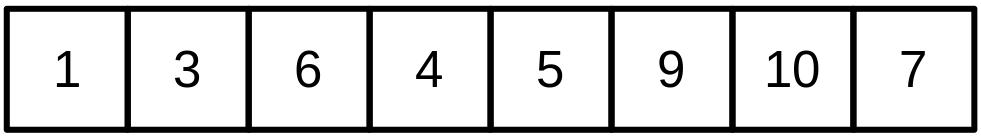
\includegraphics[width = 0.5\linewidth]{Developpements/correction tri fusion/arbre_tableau.png}}